\documentclass{beamer}
\usepackage[tohoku,zh]{collegeBeamer}
\usepackage{xeCJK}

\definecolor{hrefcol}{RGB}{0, 0, 255} % Example: blue color
\usepackage{xcolor} % For defining and using custom colors
\usepackage{natbib} % Alternative with natbib

\usepackage{natbib}
\bibliographystyle{apalike}
\setbeamercovered{transparent}

% Add your bibliography file
\bibliography{references} % For natbib
\newcommand{\rfootnote}[1]{
  \addtocounter{framenumber}{-1}
  \begin{tikzpicture}[remember picture,overlay]
    \node[anchor=south east, inner sep=2.9mm, yshift=-1mm] at (current page.south east) {
      \begin{minipage}{0.55\textwidth} % Adjust width as needed
        \tiny % Decrease font size
        #1
      \end{minipage}
    };
  \end{tikzpicture}
  \addtocounter{framenumber}{1}
}

% Define the custom color
\definecolor{custompurple}{RGB}{62,21,134}

% Define the new command for bold and colored text
\newcommand{\boldcolor}[1]{\textbf{\textcolor{custompurple}{#1}}}
% meta-data
\title{\textbf{无界抑或有界？\\在线劳动力市场中的参与壁垒与机会不平等}}
\subtitle{2024年中国社会学会社会分层与流动专业委员会冬季论坛}
\author{ \textsc{王志超}, \textsc{吕泽宇}}
\institute{%
    \textit{日本東北大学}\\
    \textit{文学研究科 \hspace{0.2cm}  计算人文社会学专攻}}

\date{2024年11月}

% document body
\begin{document}

    \maketitle

    \begin{frame}

    \begin{itemize}
        \item 本研究利用大规模的在线劳动力市场数据揭示了\boldcolor{不同国家劳动者之间不平等},并且对其形成机制进行了实证性的探讨
        \item 本研究着重关注了劳动者在\boldcolor{进入和参与在线劳动力市场初期阶段所受到的不平等}
        \begin{itemize}
            \item 发展中国家劳动者获得首次工作机会所需时间更长且所需投标次数更多,表现出出参与壁垒的不平等
        \end{itemize}
        \item 本研究探讨了劳动者的投标策略如何受到本地经济水平和市场竞争程度的限制,以及其对于不同国家间不平等的影响
    \end{itemize}

    \end{frame}

    \section{研究背景}

    \begin{frame}{长期的全球收入不平等}{\secname}
        \begin{columns}
            \begin{column}{0.5\textwidth}
            \begin{figure}
            \centering
            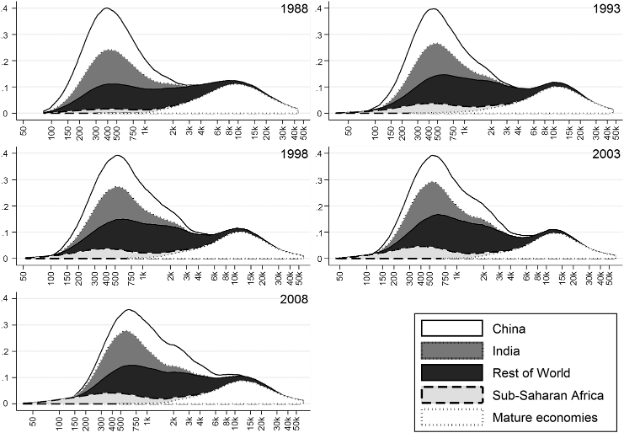
\includegraphics[width=\linewidth]{incom_inequality.png}
            \caption{The Global Distribution of Income\\(Lakner and Milanovic 2015)}
            \label{fig:enter-label}
            \end{figure}
            \end{column}
            \begin{column}{0.5\textwidth}
                \begin{itemize}
                    \item 长期以来, \textbf{不同国家和地区之间的收入水平存在显著的不平等}
                    \pause
                    \item \textbf{地理障碍对劳动力流动的限制}:传统工作形态通常要求劳动者在物理上靠近工作地点
                    \begin{itemize}
                        \item 劳动者的机会受限于本地市场的规模与需求
                        \item 劳动力的供给（劳动者技能）与需求（岗位要求）的地理错配
                    \end{itemize}

                \end{itemize}
            \end{column}
        \end{columns}
    \rfootnote{Lakner, Christoph, and Branko Milanovic. 2015. “Global Income Distribution: From the Fall of the Berlin Wall to the Great Recession.” The World Bank Economic Review 30 (2): 203–32.}
    \end{frame}

    \begin{frame}{在线劳动力市场的基本运作模式}{\secname}
        \begin{columns}
            \begin{column}{0.5\textwidth}
            \begin{figure}
        \centering
        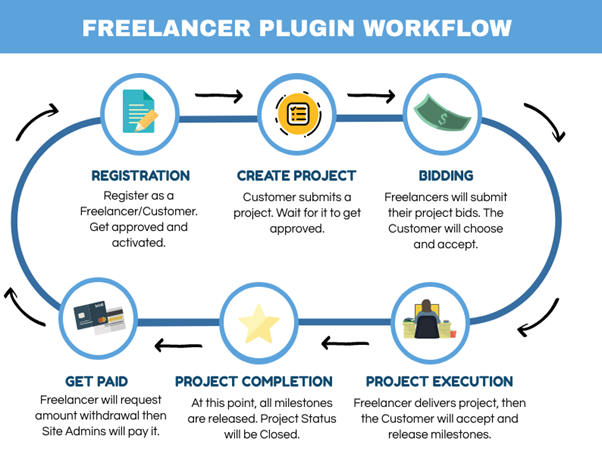
\includegraphics[width=\linewidth]{flowchart.png}
        \caption{在线劳动力市场的基本运作形式}
        \label{fig:enter-label}
        \end{figure}
            \end{column}
            \begin{column}{0.5\textwidth}
                \begin{itemize}
                    \item 雇主发布任务
                    \begin{itemize}
                        \item 包括工作描述、目标、所需技能、预计工作量以及预算
                    \end{itemize}
                    \pause
                    \item 劳动者响应并提交投标
                    \pause
                    \item 竞争与筛选
                    \pause
                    \begin{itemize}
                        \item 多名劳动者可能会对同一任务投标，由雇主进行选择
                    \end{itemize}
                    \item 报酬支付与反馈
                    \begin{itemize}
                        \item 劳动者和雇主互相评价，建立个人信誉
                    \end{itemize}

                \end{itemize}
            \end{column}
        \end{columns}

    \end{frame}

    \begin{frame}{在线劳动力市场中的不平等}{\secname}
    \begin{itemize}
    \pause
        \item \textbf{在线劳动力市场缓和劳动力市场中不平等现象的可能性}(Beerepoot\&Lambregts 2015; Manyika et al. 2015)
        \begin{itemize}
            \item 降低准入门槛
            \item 灵活的工作方式
            \item 透明度和技能优先的竞争机制
        \end{itemize}
        \pause
        \item \textbf{在线劳动力市场中仍呈现出与线下劳动力市场类似的结构性不平等}(Hong et al. 2017; Galperin\&Greppi 2019; Slageren et al. 2023)
        \begin{itemize}
            \item 性别 (Chan \& Wang, 2018;Litman et al., 2020)
            \item 种族 ((Maurer-Fazio, 2012;)
        \end{itemize}
    \end{itemize}
    \pause
    \begin{block}{RQ1}
        \begin{itemize}
            \item \textbf{在线劳动力市场是否缓和了不同经济发展水平国家劳动者间的收入不平等?}
        \end{itemize}
    \end{block}
    \end{frame}
    
    \begin{frame}{收入不平等的形成中初期过程的影响}{\secname}
    \begin{itemize}
    \pause
        \item \textbf{初始阶段中的自身定位:参照群体的选择}
        \begin{itemize}
            \item 以在线劳动力市场的报酬水平为参照
            \item 以所处地区的收入水平为参照
        \end{itemize}
        \pause
        \item \textbf{初期过程的长期影响}
        \begin{itemize}
            \item \textbf{反馈循环与路径依赖}: 早期反馈（例如投标成功或失败、工作类型和职位质量）会形成路径依赖效应影响劳动者的自我定位和职业选择
            \item \textbf{累积劣势的机制}: 初期阶段的不利条件通过时间逐步累积形成持续的结构性劣势
        \end{itemize}
    \end{itemize}
    \pause
    \begin{block}{RQ2}
        \begin{itemize}
            \item \textbf{不同经济发展水平国家劳动者在参与在线劳动力市场初期呈现了怎么样的行为特征?}
        \end{itemize}
    \end{block}
    \end{frame}    
    


    \section{数据和方法}
    \begin{frame}{数据概要}{\secname}
        \begin{columns}
            \begin{column}{0.6\textwidth}
            \begin{figure}
            \centering
            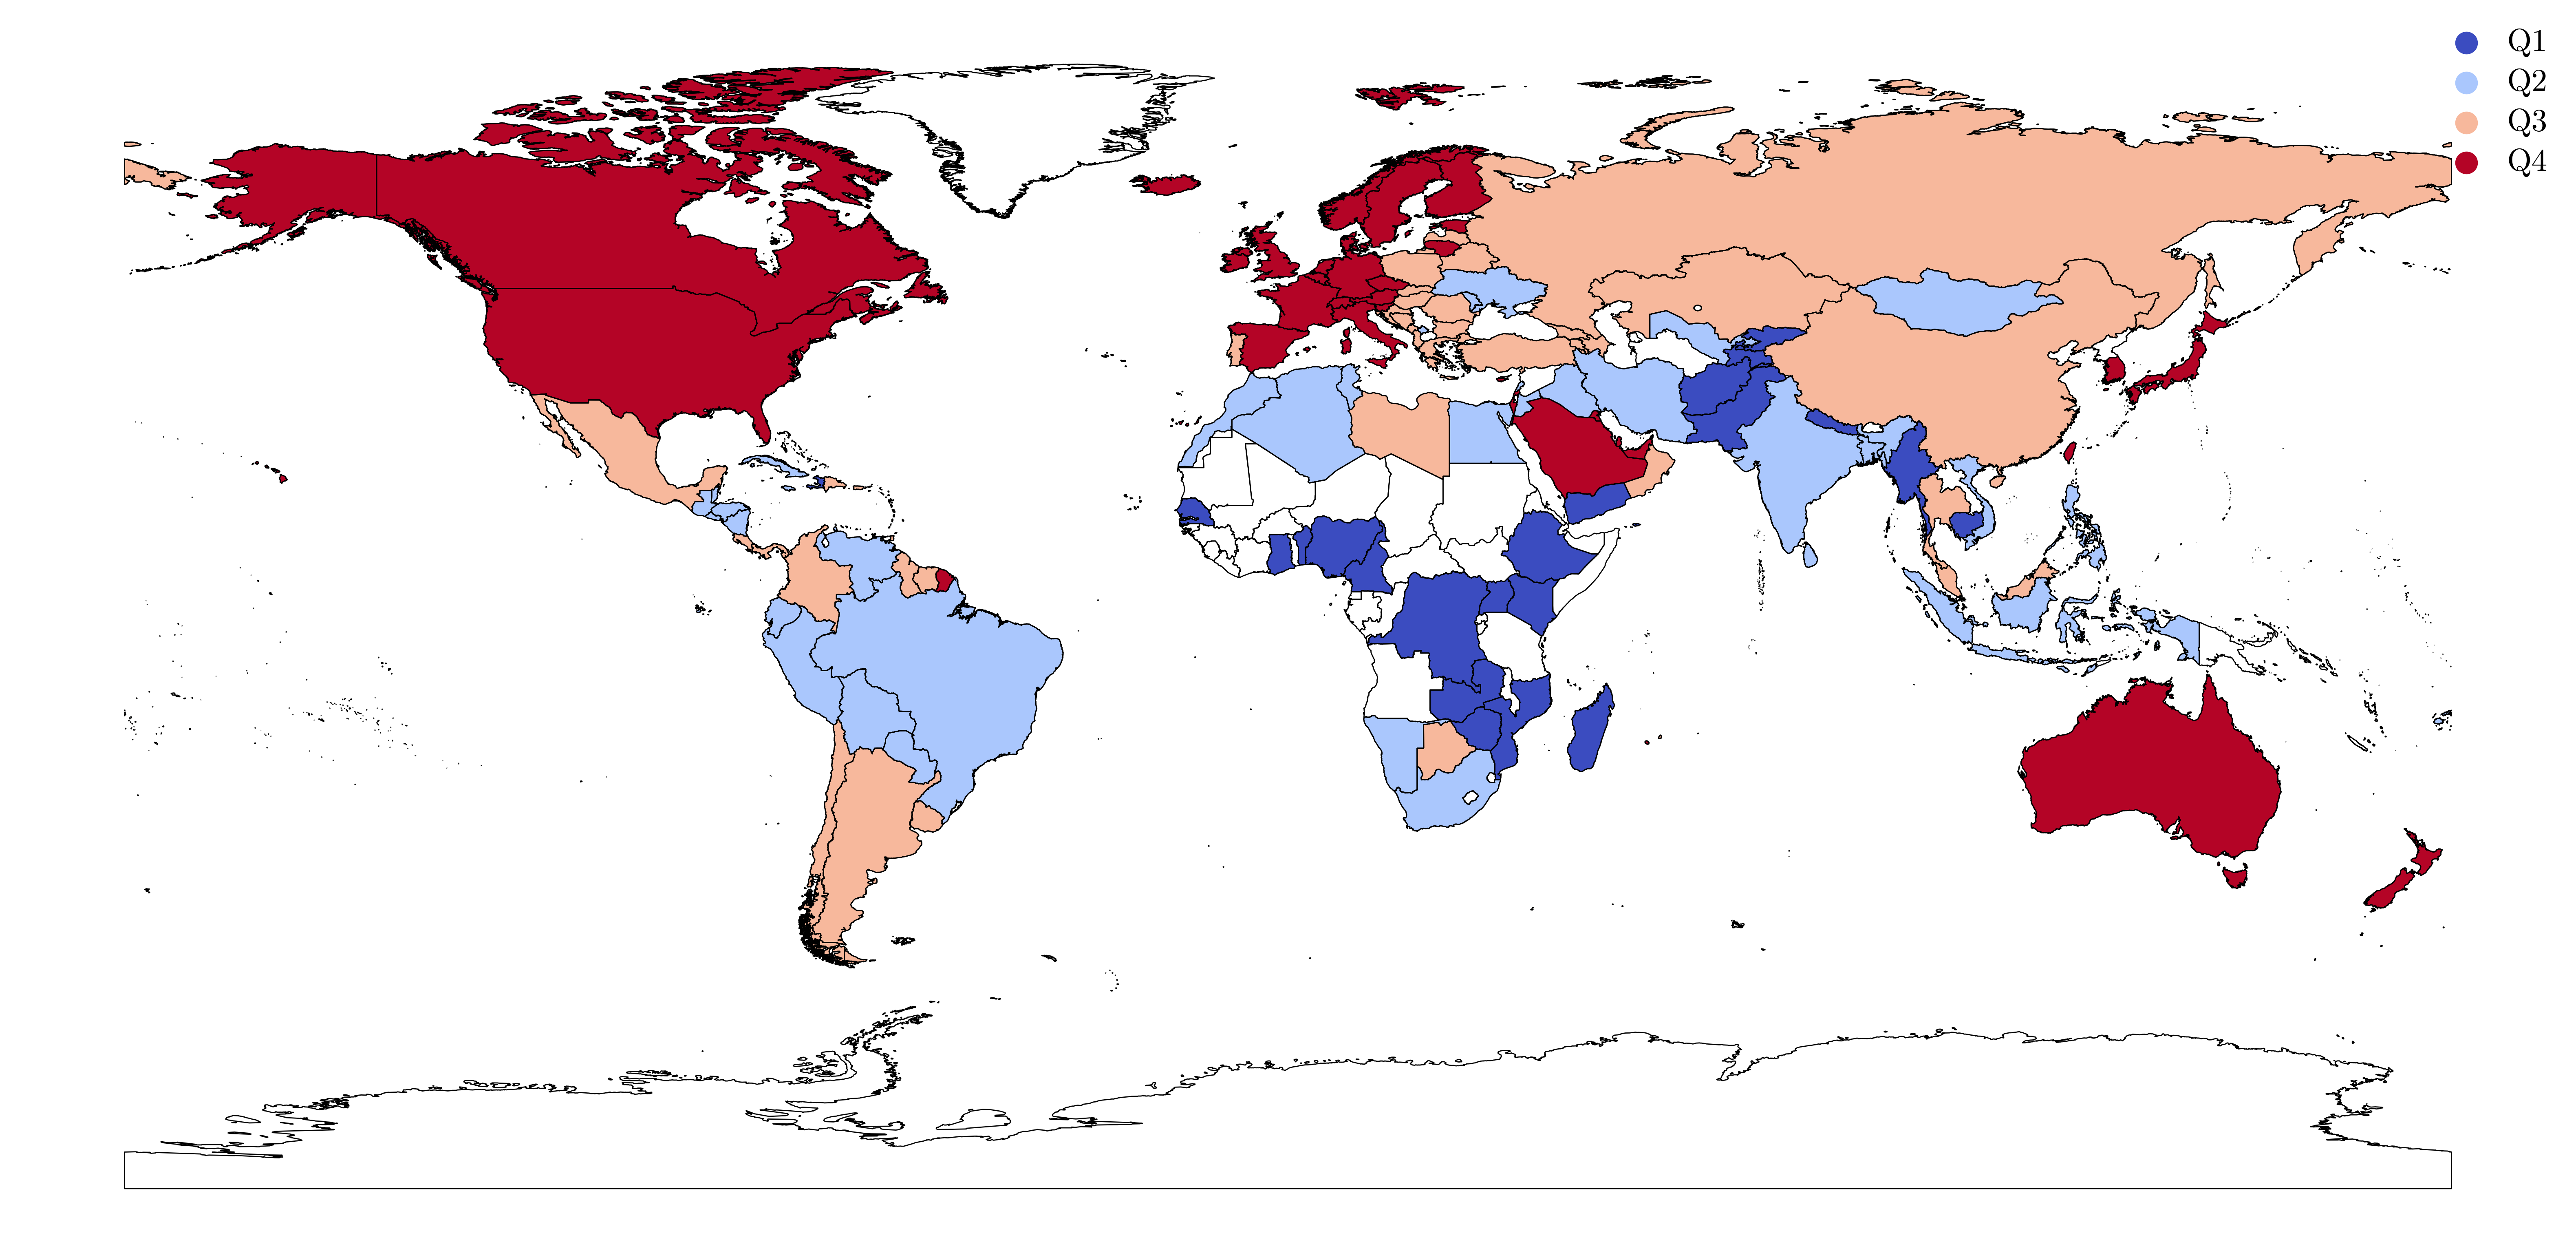
\includegraphics[width=\linewidth]{map.png}
            \caption{\textit{Freelancer}用户的国家及其经济发展水平}
            \label{fig:enter-label}
            \end{figure}
        \end{column}
        \begin{column}{0.4\textwidth}
                \begin{itemize}
                    \item 2014年1月至2017年1月期间\textit{Freelancer}在线劳动力市场数据
                    \begin{itemize}
                        \item N=673,479活跃劳动者的平台信息
                        \item N=1,971,601招聘信息
                        \item N=8,581,070投标行为
                    \end{itemize}
                    \item 覆盖了全世界大部分\boldcolor{不同经济发展水平的国家}
                \end{itemize}
            \end{column}
        \end{columns}
    \end{frame}


    \begin{frame}{数据结构}{\secname}
    \begin{minipage}[t]{0.3\textwidth} % 第1列，占30%宽度
        \boldcolor{劳动者信息}
            \begin{itemize}
                \item 所在国家
                \item 期望薪资
                \item 项目经历
                \item ...
            \end{itemize}
    \end{minipage}%
    \hfill % 添加水平间距
    \begin{minipage}[t]{0.3\textwidth} % 第2列，占30%宽度
    \boldcolor{招聘信息}
            \begin{itemize}
                \item 预期报酬
                \item 实际报酬
                \item 工作内容类型
                \item ...
            \end{itemize}
    \end{minipage}%
    \hfill % 添加水平间距
    \begin{minipage}[t]{0.3\textwidth} % 第3列，占30%宽度
    \boldcolor{投标行为信息}
            \begin{itemize}
                \item 竞标价格信息
                \item 竞标者信息
                \item 中标者信息
                \item ...
            \end{itemize}
    \end{minipage}
    \pause
    \begin{block}{数据的优势和特点}
        \begin{itemize}
            \item 捕捉了在线劳动力市场中多角度的长期动态变化
            \item 了解在线劳动力市场之中不同主体之间的互动关系
        \end{itemize}
    \end{block}
    \end{frame}

    \begin{frame}{分析方法}{\secname}
    \begin{itemize}
        \item 利用大规模的实证数据描述在线劳动力市场中不同经济发展水平国家劳动者之间的不平等
        \begin{itemize}
            \item 收入不平等
            \item \textbf{参与壁垒和机会的不平等}
        \end{itemize}
        \item 劳动力市场参与初期阶段劳动者的投标策略及其变动
        \begin{itemize}
            \item 分析不同经济发展水平国家的首次投标价格的差异
            \item 不同经济发展水平国家之间投标价格不平等的动态变化
        \end{itemize}
    \end{itemize}
    \end{frame}
    
    \section{分析结果}

    \begin{frame}{不同国家劳动者之间获取报酬的不平等}{\secname}
        \begin{columns}
            \begin{column}{0.6\textwidth}
            \begin{figure}
            \centering
            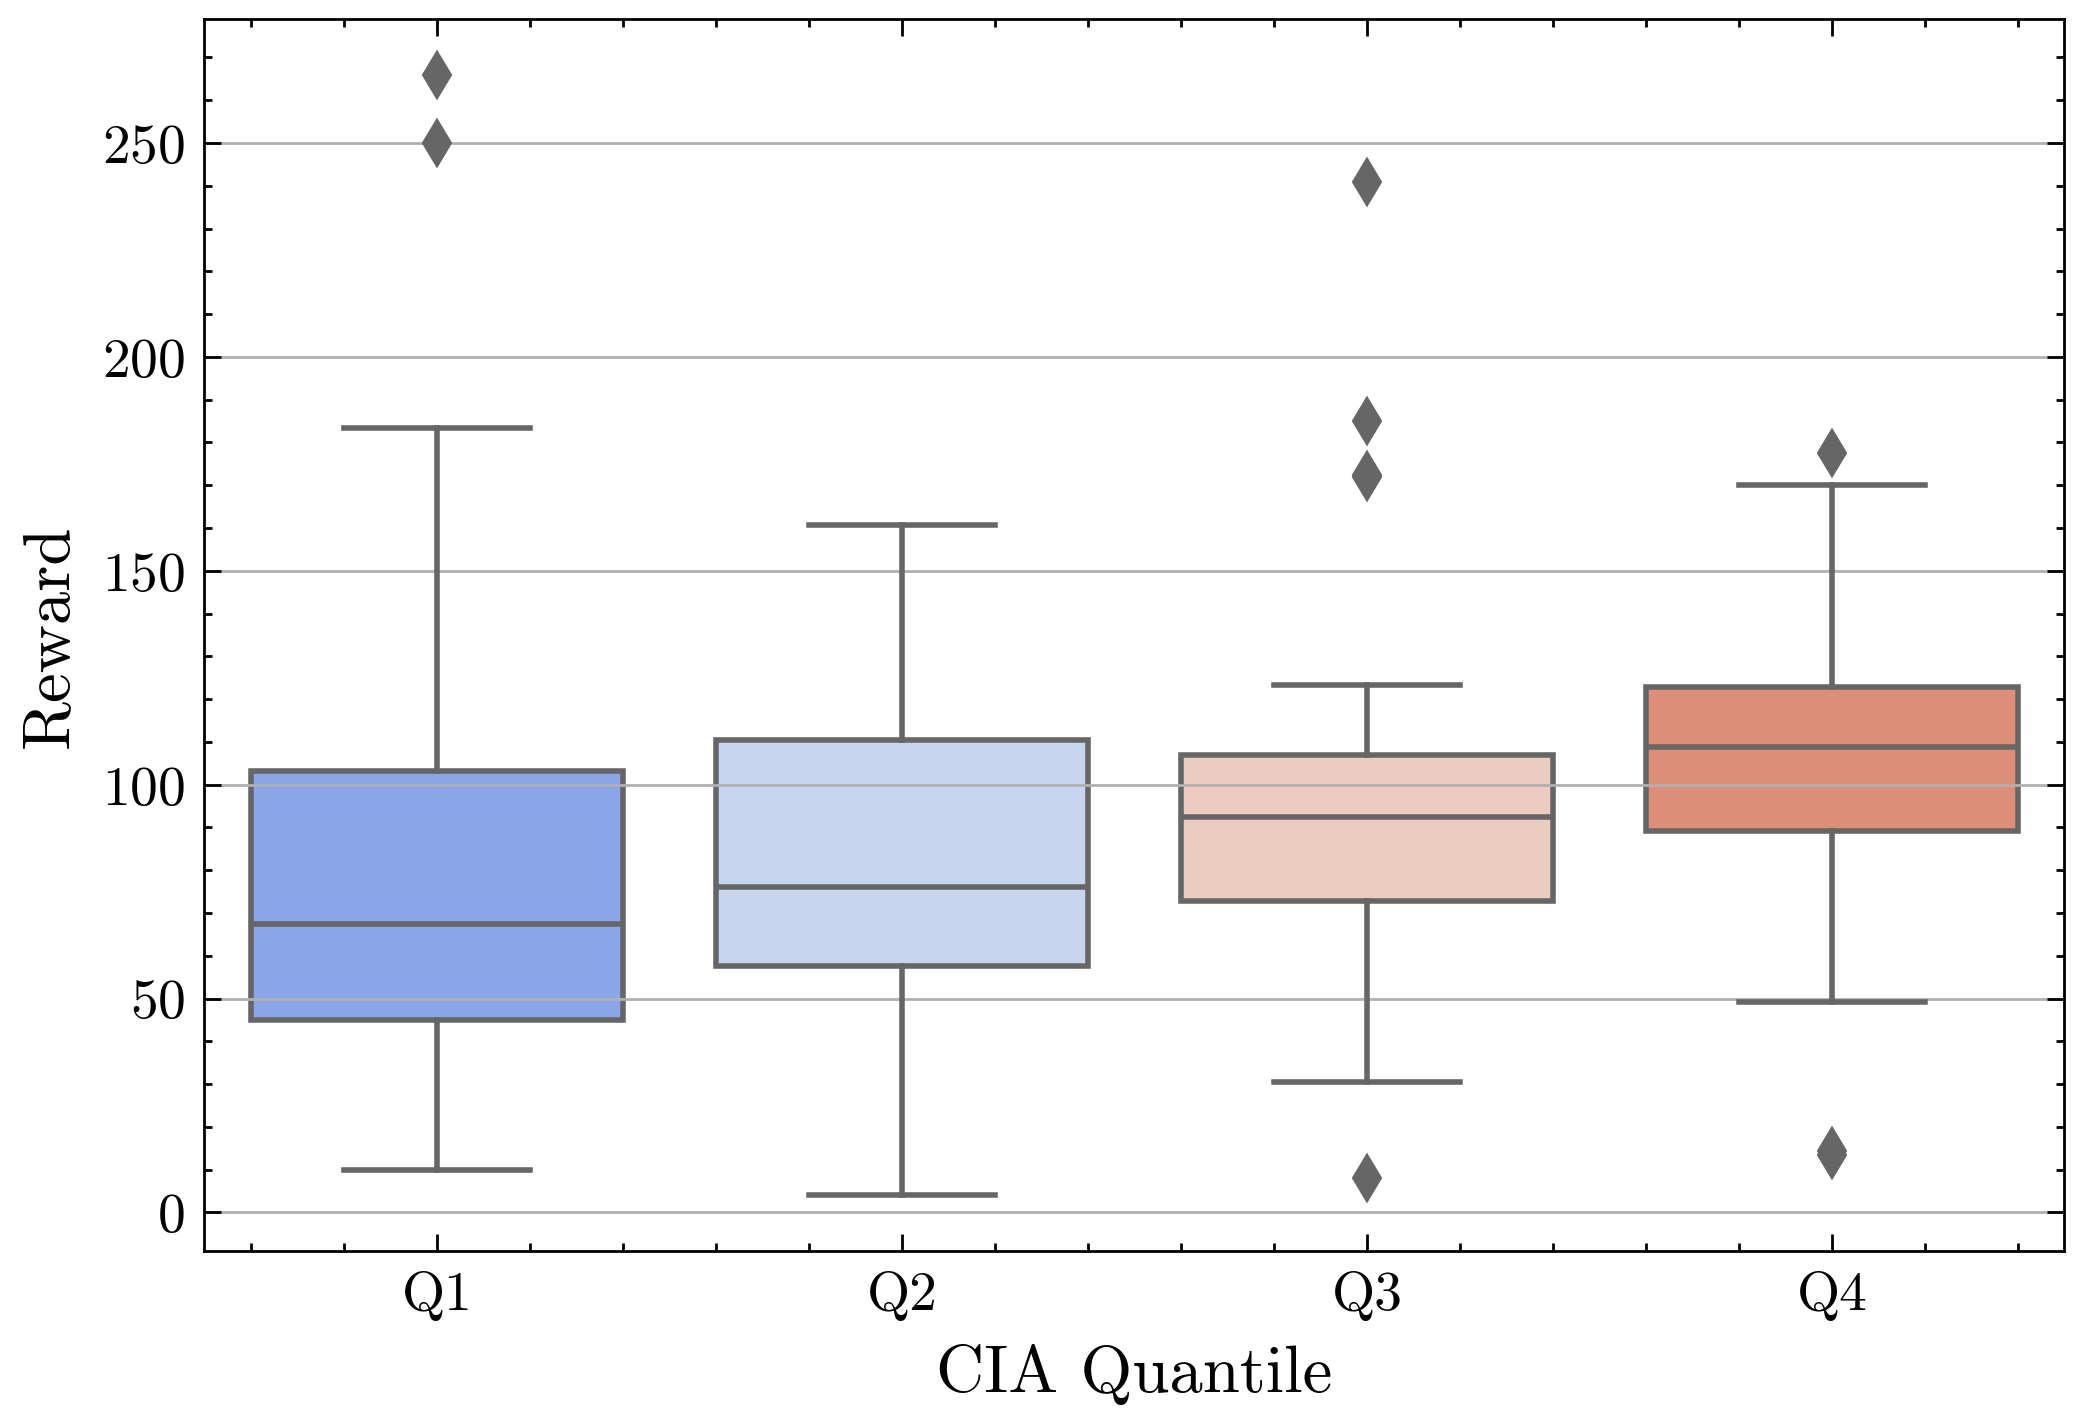
\includegraphics[width=\linewidth]{reward_inequality.png}
            \caption{不同经济发展水平国家间获取报酬的差异}
            \label{fig:enter-label}
            \end{figure}
        \end{column}
        \begin{column}{0.4\textwidth}
                \begin{itemize}
                \item 在线劳动力市场中，来自高经济发展水平国家的劳动者通常能够获得更高的报酬
                \begin{itemize}
                    \item 体现了全球劳动力市场中存在的结构性不平等在在线劳动力市场中的映射
                \end{itemize}

                \end{itemize}
            \end{column}
        \end{columns}
       \end{frame}


    \begin{frame}{不同国家劳动者之间期望报酬的不平等}{\secname}
        \begin{columns}
            \begin{column}{0.5\textwidth}
            \begin{figure}
            \centering
            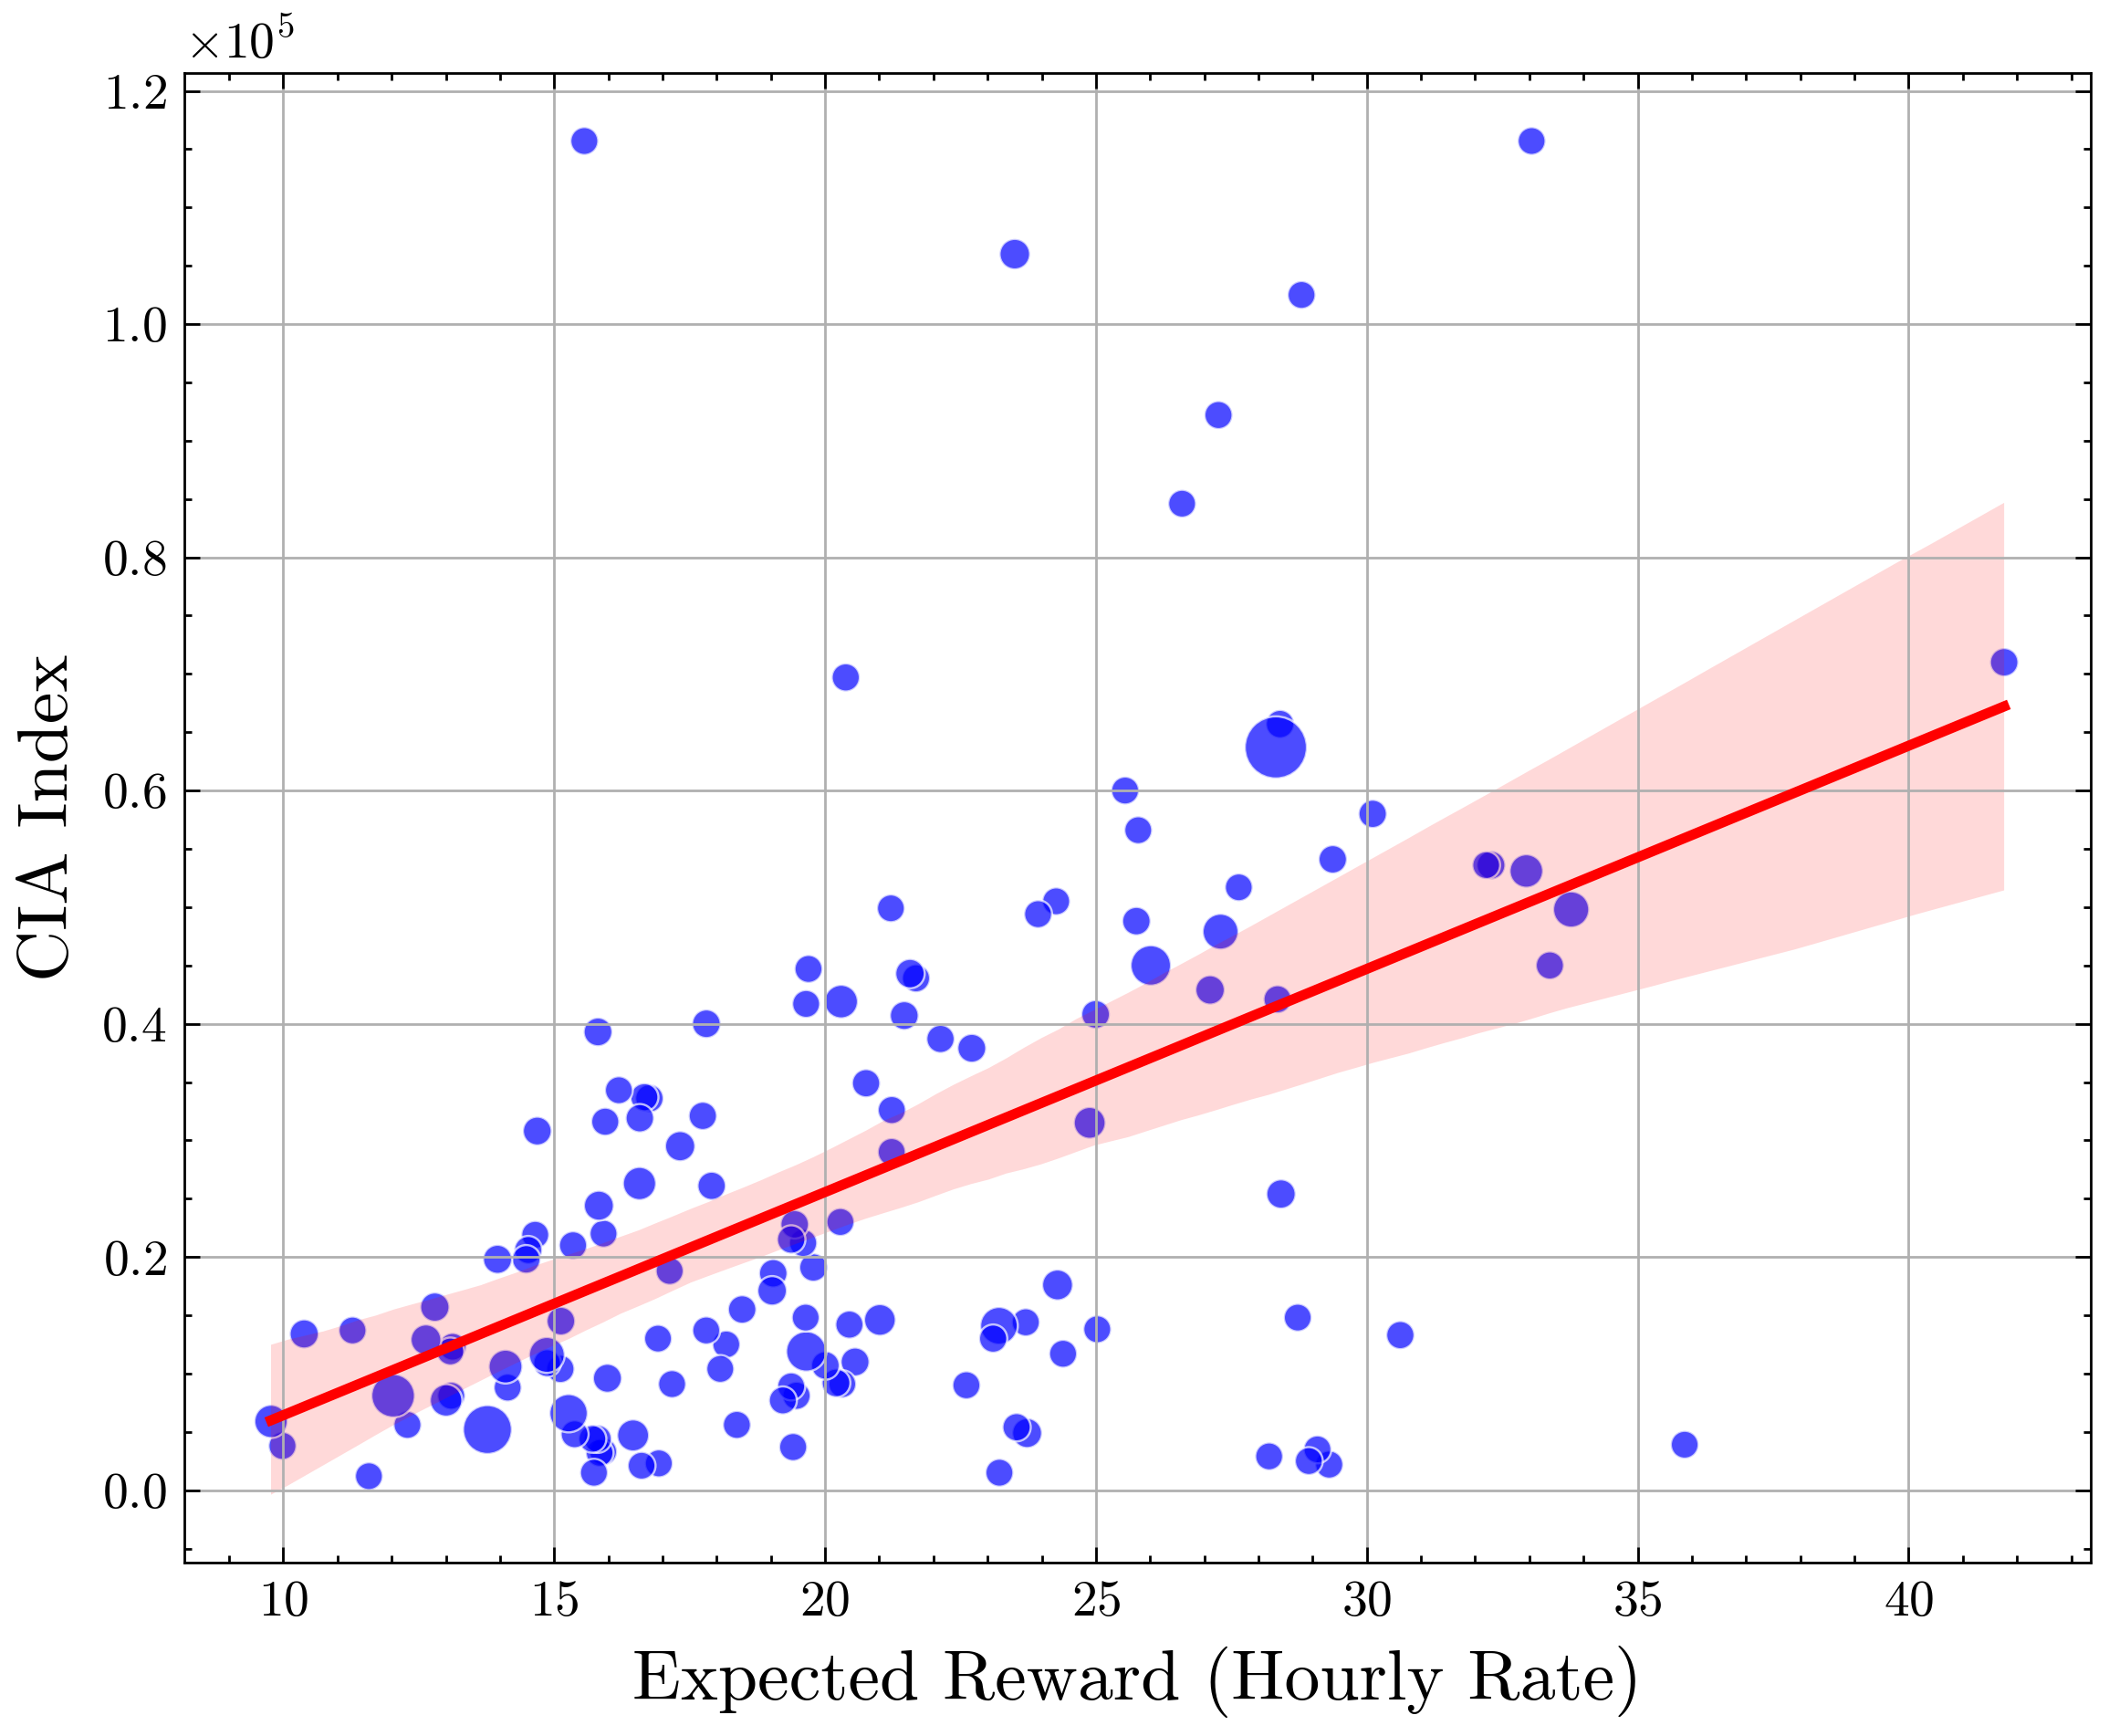
\includegraphics[width=0.8\linewidth]{Expected_Reward_CIA.png}
            \caption{期望报酬和国家经济发展水平的关系}
            \label{fig:enter-label}
            \end{figure}
        \end{column}
        \begin{column}{0.5\textwidth}
                \begin{itemize}
                \item 国家的经济发展水平与劳动者的期望报酬呈现正相关
                %\begin{itemize}
                %    \item 期望报酬: 每小时回报率
                %    \item 国家的经济发展水平: CIA指数
                %\item 济发展水平不平等的结构性因素制约
                \item 经济发展水平不平等的结构性因素制约
                \begin{itemize}
                    \item 劳动者倾向于将其国家经济环境中的工资水平作为心理锚点
                    \item 基于隐性偏见而形成的国家间经济发展水平的不平等再生产
                \end{itemize}

                \end{itemize}
            \end{column}
        \end{columns}
    \end{frame}






    \begin{frame}{不同国家劳动者之间参与壁垒的不平等}{\secname}

            \begin{figure}
            \centering
            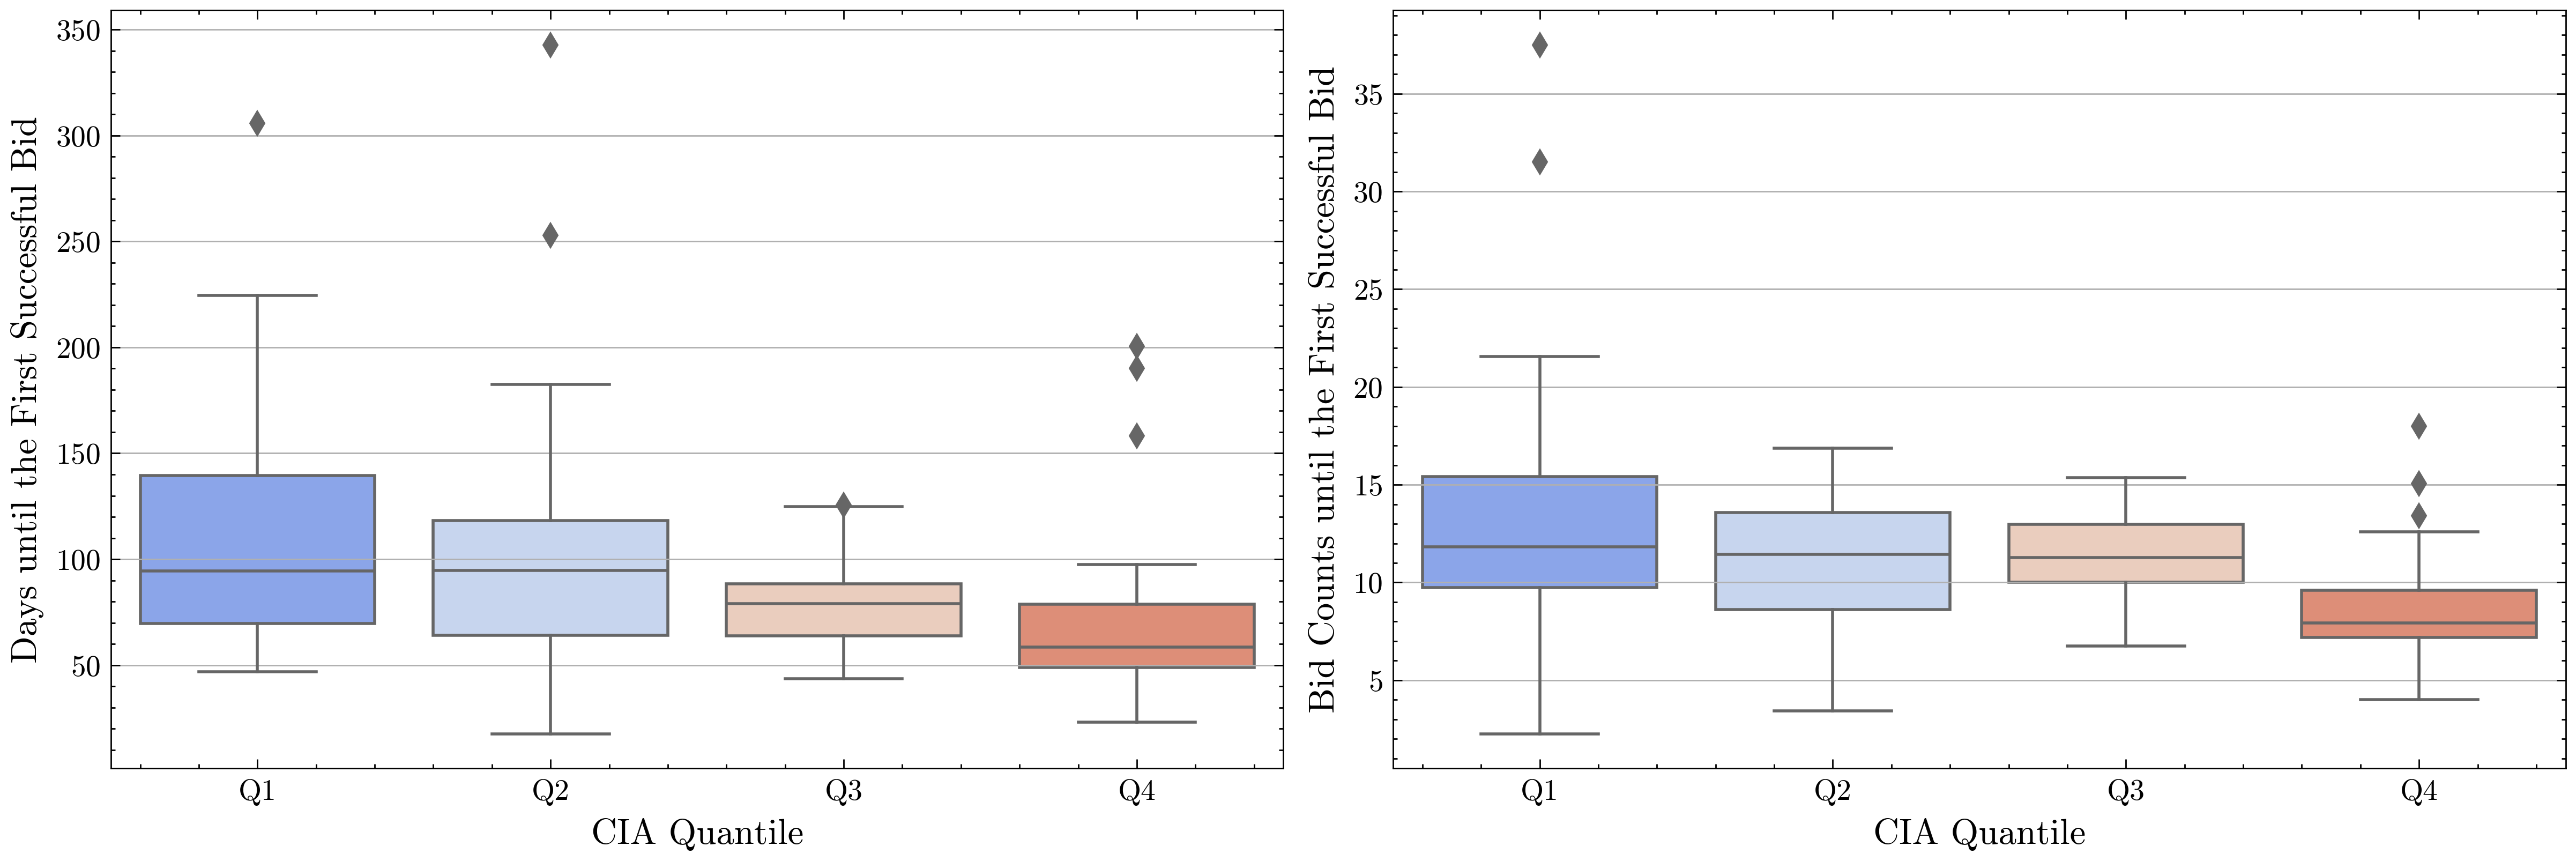
\includegraphics[width=\linewidth]{First_inequality.png}
            \caption{不同经济发展水平国家劳动者的参与壁垒}
            \label{fig:enter-label}
            \end{figure}

       \end{frame}

    \begin{frame}{不同国家劳动者初次投标策略的差异}{\secname}
        \begin{columns}
            \begin{column}{0.45\textwidth}
            \begin{figure}
            \centering
            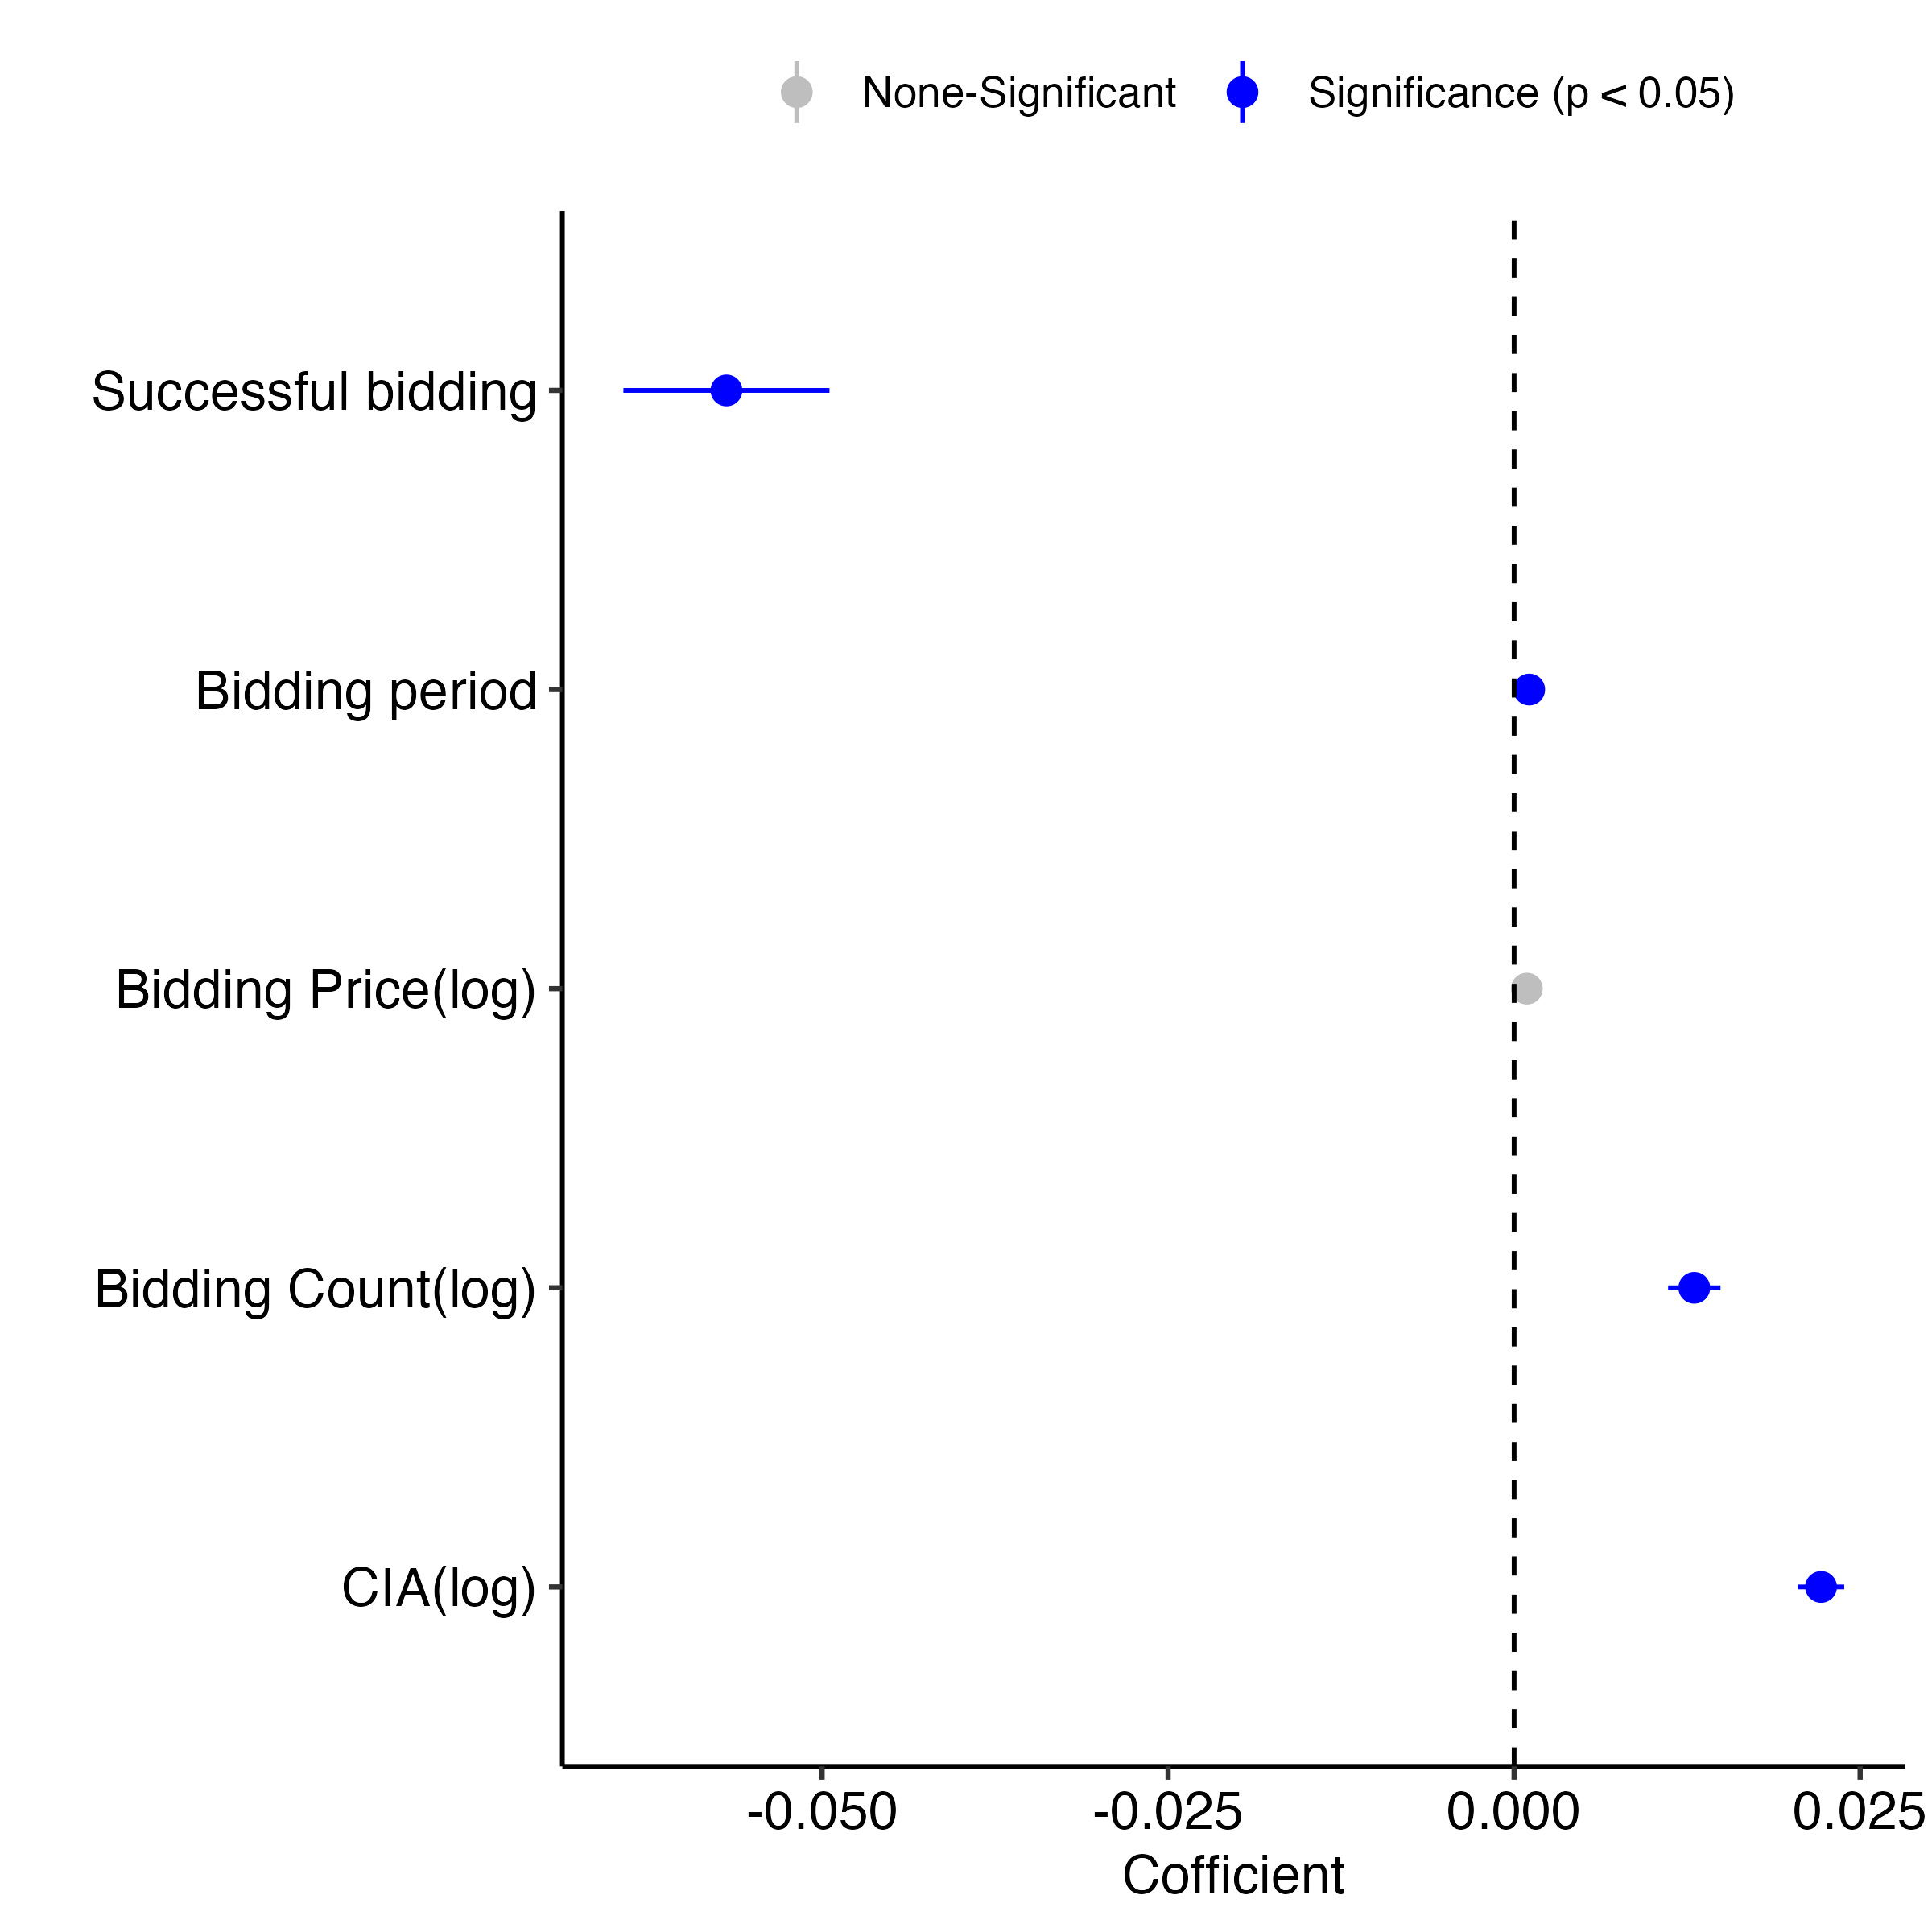
\includegraphics[width=0.9\linewidth]{first_bidding_regression_plot.png}
            \caption{初次投标的影响因素}
            \label{fig:enter-label}
            \end{figure}
        \end{column}
        \begin{column}{0.53\textwidth}
                \begin{itemize}
                \item 在统制了投标的相关因素的基础上验证国家经济发展水平对于初次投标价格设定的影响
                \begin{itemize}
                    \item \textbf{自变量: 国家经济发展水平(CIA)}
                    \item \textbf{因变量: 投标价格与雇主预算的比例}
                    \item 统制变量: 投标期间, 投标均价, 投标数量,是否中标
                \end{itemize}

                \end{itemize}
            \end{column}
        \end{columns}
       \end{frame}

    \begin{frame}{不同国家劳动者初次投标策略的差异}{\secname}
        \begin{columns}
            \begin{column}{0.45\textwidth}
            \begin{figure}
            \centering
            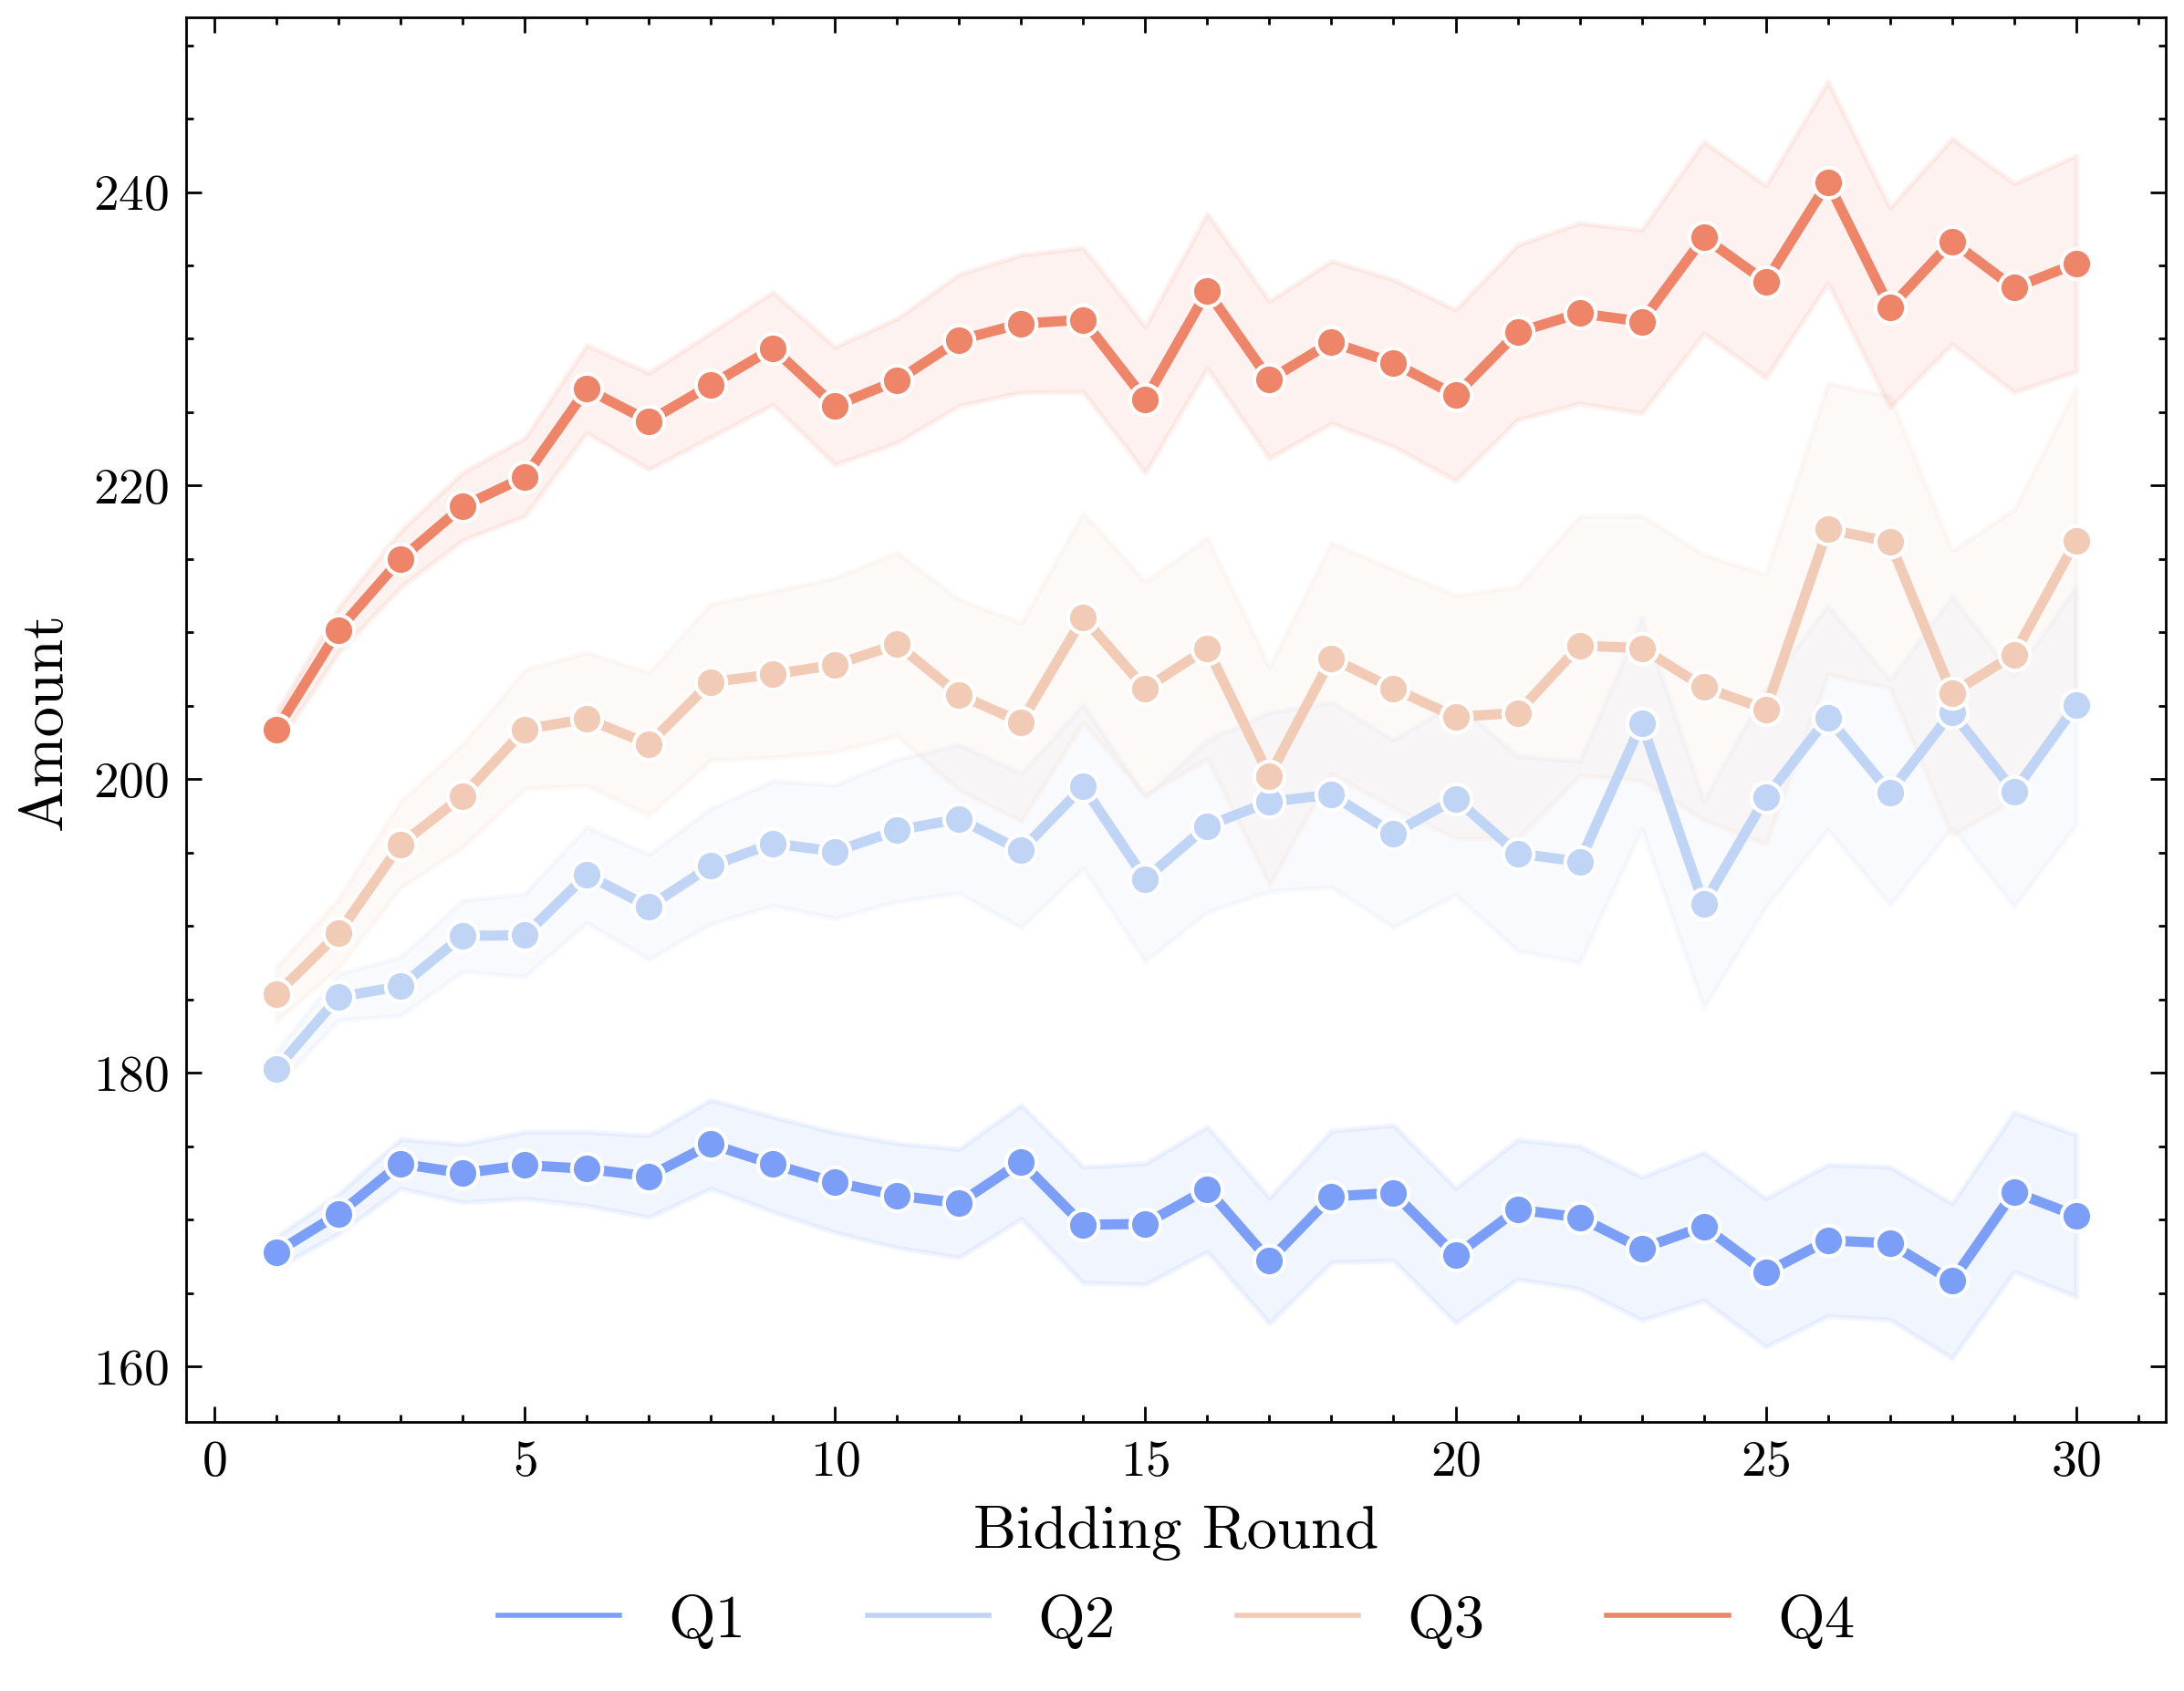
\includegraphics[width=0.9\linewidth]{bidding_round.png}
            \caption{不同经济发展水平国家劳动者的投标价格变动}
            \label{fig:enter-label}
            \end{figure}
        \end{column}
        \begin{column}{0.53\textwidth}
        \begin{figure}
            \centering
            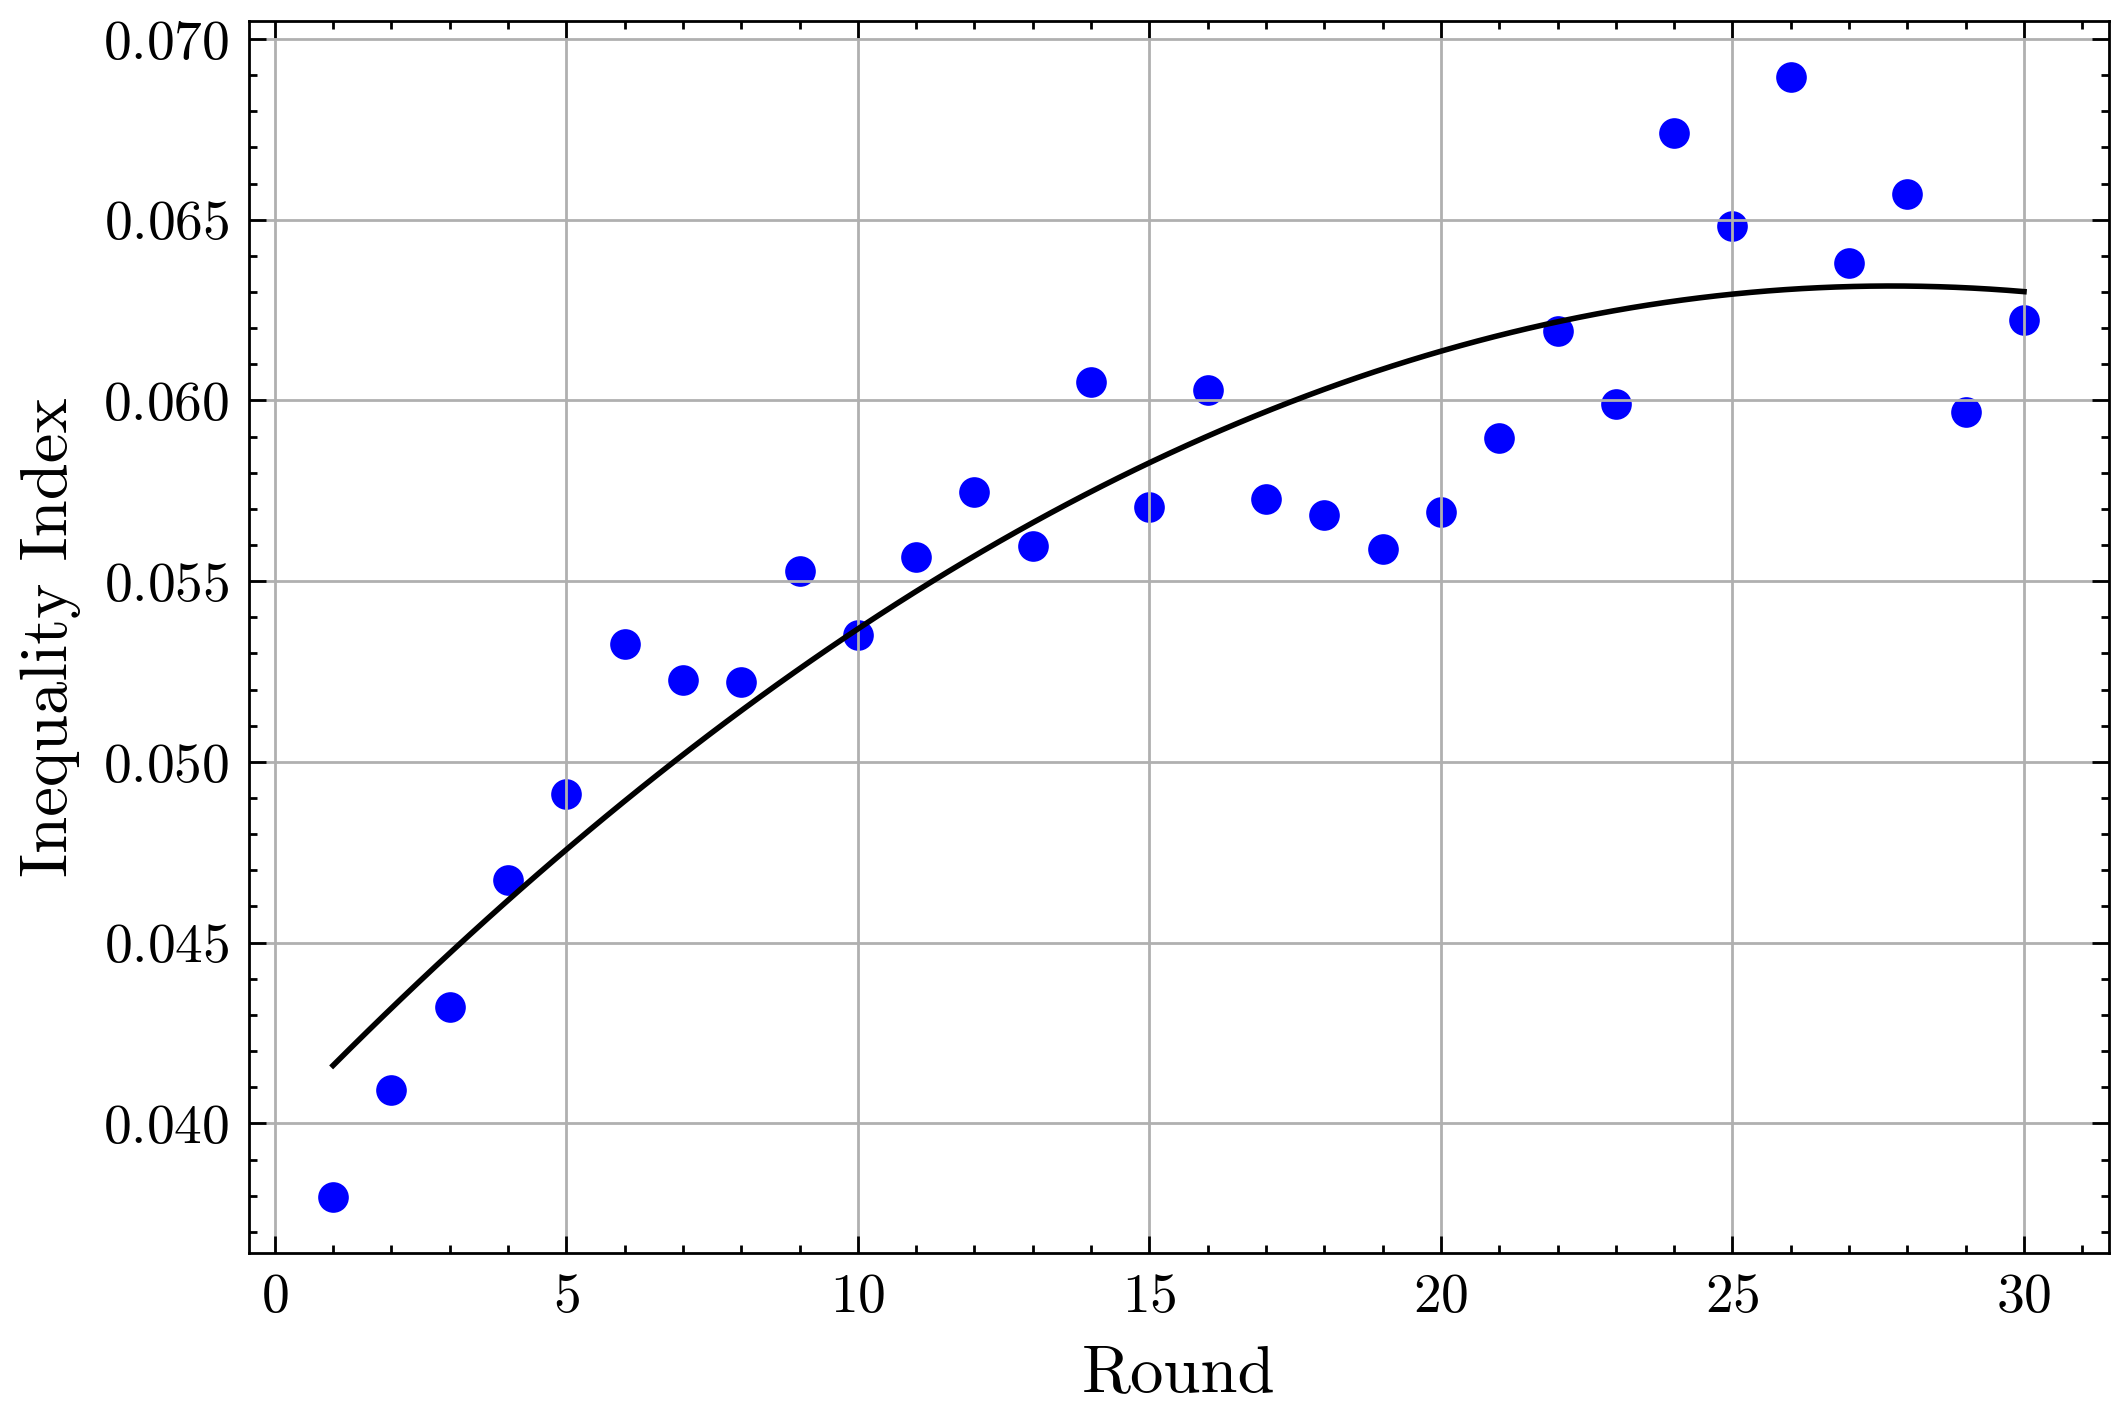
\includegraphics[width=0.9\linewidth]{inequality.png}
            \caption{不同经济发展水平国家劳动者的投标价格不平等程度的变化}
            \label{fig:enter-label}
            \end{figure}
  
            \end{column}
        \end{columns}
       \end{frame}
       
    \section{总结与讨论}
    
        \begin{frame}{不同国家劳动者之间不平等形成和扩大的机制}{\secname}

        \begin{itemize}
            \item \textbf{劳动者的期望薪资的差异体现了不同国家经济发展水平在在线劳动力市场层面的映射}
            \begin{itemize}
                \item 劳动者的期望薪资影响了其首次投标的价格
            \end{itemize}
            \pause
            \item \textbf{在线劳动力市场中的负面反馈会造成不平等的扩大}
            \begin{itemize}
                \item 来自不同经济发展水平国家的劳动者在初期阶段的参与壁垒和机会不平等影响了其投标价格策略
            \end{itemize}
        \end{itemize}

       \end{frame}




    \QApage

\end{document}
